% Options for packages loaded elsewhere
\PassOptionsToPackage{unicode}{hyperref}
\PassOptionsToPackage{hyphens}{url}
%
\documentclass[
]{article}
\usepackage{lmodern}
\usepackage{wrapfig}
\usepackage{subcaption}
\usepackage{graphicx}
\usepackage{amssymb,amsmath}
\usepackage{ifxetex,ifluatex}
\ifnum 0\ifxetex 1\fi\ifluatex 1\fi=0 % if pdftex
  \usepackage[T1]{fontenc}
  \usepackage[utf8]{inputenc}
  \usepackage{textcomp} % provide euro and other symbols
\else % if luatex or xetex
  \usepackage{unicode-math}
  \defaultfontfeatures{Scale=MatchLowercase}
  \defaultfontfeatures[\rmfamily]{Ligatures=TeX,Scale=1}
\fi
% Use upquote if available, for straight quotes in verbatim environments
\IfFileExists{upquote.sty}{\usepackage{upquote}}{}
\IfFileExists{microtype.sty}{% use microtype if available
  \usepackage[]{microtype}
  \UseMicrotypeSet[protrusion]{basicmath} % disable protrusion for tt fonts
}{}
\makeatletter
\@ifundefined{KOMAClassName}{% if non-KOMA class
  \IfFileExists{parskip.sty}{%
    \usepackage{parskip}
  }{% else
    \setlength{\parindent}{0pt}
    \setlength{\parskip}{6pt plus 2pt minus 1pt}}
}{% if KOMA class
  \KOMAoptions{parskip=half}}
\makeatother
\usepackage{xcolor}
\IfFileExists{xurl.sty}{\usepackage{xurl}}{} % add URL line breaks if available
\IfFileExists{bookmark.sty}{\usepackage{bookmark}}{\usepackage{hyperref}}
\hypersetup{
  pdftitle={Network robustness and percolation theory},
  pdfauthor={Spina Lorenzo, Piermarco , Trapanotto Martino},
  hidelinks,
  pdfcreator={LaTeX via pandoc}}
\urlstyle{same} % disable monospaced font for URLs
\usepackage{graphicx}
\makeatletter
\def\maxwidth{\ifdim\Gin@nat@width>\linewidth\linewidth\else\Gin@nat@width\fi}
\def\maxheight{\ifdim\Gin@nat@height>\textheight\textheight\else\Gin@nat@height\fi}
\makeatother
% Scale images if necessary, so that they will not overflow the page
% margins by default, and it is still possible to overwrite the defaults
% using explicit options in \includegraphics[width, height, ...]{}
\setkeys{Gin}{width=\maxwidth,height=\maxheight,keepaspectratio}
% Set default figure placement to htbp
\makeatletter
\def\fps@figure{htbp}
\makeatother
\setlength{\emergencystretch}{3em} % prevent overfull lines
\providecommand{\tightlist}{%
  \setlength{\itemsep}{0pt}\setlength{\parskip}{0pt}}
\setcounter{secnumdepth}{-\maxdimen} % remove section numbering

\title{Network robustness and percolation theory}
\author{Spina Lorenzo, Piermarco , Trapanotto Martino}
\date{October 27, 2022}

\begin{document}
\maketitle

\hypertarget{introduction}{%
\section{Introduction}\label{introduction}}

In this work, we want to try and tackle the topic of network robustness,
both for random networks and for more realistic network topologies.

With the term robustness, we mean the capacity of a network to keep it's
connected nature under node failure, both randomized and targeted. This
should be a reasonable way to approach the idea of the resilience of a
network to both random failure of components and targeted attacks, and
allow us to lay the groundwork for more advanced studies, such as
enhancing robustness, recognizing more vulnerable or higher priority
targets and more.

To analyze the topic, we'll use the conceptual and mathematical
framework defined by Percolation Theory, a branch of mathematics that
studies the evolution on networks when nodes and edges are added.

\hypertarget{percolation-theory}{%
\section{Percolation Theory}\label{percolation-theory}}

The origin of the name stems from the question posed in the 1957 paper
that originated the filed: If liquid is poured of a porous material,
does the liquid flow through the cavities until reaching the bottom?

Percolation theory models this phenomenon as a 3D lattice structure
where nodes represent holes in the material and links possible passages
between these cavities. Thus, creating a statistical model for the
porous material.

The filed has expanded as a branch of mathematics and statistical
physics and is quite richly explored, with applications now ranging in
ecology, biology, biochemistry, virology, statistical modeling and, as
we'll show, network science.

\hypertarget{lattices-and-networks}{%
\subsection{Lattices and networks}\label{lattices-and-networks}}

{[}Check wording, perhaps some basic images of percolation structures{]}

Lattices are the most common model used in percolation theory,
constructing a regular network where nodes are connected only to their
relative neighbors in a regular pattern. These can be square, triable,
hexagon, 2D, 3D, 4D.

All these share some common properties, given by the number of
dimensions. The parameters that define these properties are called
\emph{Critical Exponents}.

These networks are generated by placing the nodes in our lattice, and
associating the edges with a random \(X_i \thicksim Ber(p)\) variable.
Each edge exists only if \(X_i = 1\), so each edge has the same
probability \(p\) of existing.

One of the key findings of percolation theory is that many key
properties of the generated graph, such as average cluster size or
likelihood of reachability between nodes, are not linked directly with
the evolution of \(p\). Instead, there is a key value \(p_c\) called
\emph{Critical probability}, and when \(p>p_c\) the network structure
changes: The smaller cluster connect and a major network component,
usually called \emph{percolating cluster}, appears and connects the
majority of the network.

Here, the role of the critical exponents can become much clearer: \[
\begin{aligned}
d &\thicksim \lvert p-pc \lvert ^{-\gamma_p} \\
p_{\infty}&\thicksim(p-pc)^{\beta_p} \\
\xi&\thicksim \lvert p-pc \lvert ^{-\nu}
\end{aligned}
\]

These three equations connect our probability \(p\) with the properties:

\begin{itemize}
\item
  d - Average Cluster Size
\item
  \(P_\infty\) - Order Parameter: probability that single node connects
  to the percolation cluster
\item
  \(\xi\) - Correlation Length: average distance between members of the
  same cluster
\end{itemize}

So, the network evolves quickly into a large unified structure when the
\(p_c\) threshold is crossed.

Conversely, this process can be looked in reverse, starting from a fully
formed and connected network: removing nodes with a small probability
\(f\), until the major connected component fails, and the network is
completely shattered.

This allows us to reframe the problem of network robustness into a
percolation problem.

Much like the creation process, this \emph{Inverse Percolation} is not a
smooth process but an abrupt one, where the network can reroute most
connections and paths until a value \(f_c = 1-p_c\) called
\emph{Critical Threshold}, is reached and the network collapses.

All these processes and the values governing them can be computed for
the aforementioned lattices, but have also been studied and analyzed for
other topologies, such as random networks or Scale-Free models. This
allows Percolation theory to model failures over a wide range of network
types.

To model the interconnectedness of the network we'll consider only one
of the previously identified parameters: \(P_\infty\), more specifically
the ratio \(\Large \frac{P_{\infty}(f)}{P_{\infty}(0)}\) comparing the
original network's Order Parameter to the value after a removal with
probability \(f\).

We'll also be computing the Molly-Reed Criterion, which allows us to
estimate analytically the critical threshold parameter, comparing it
with our empirical results.

{[}ugly passage{]} The last component to introduce is the distribution
\(k\) of the degrees of the nodes, of which we'll use different values
like moments or maximum values in various occurrences.

In the rest of the work we'll be showing the results of these analyses
for various types of networks and verifying the theoretical results on
both artificial and real datasets.

\hypertarget{random-networks}{%
\section{Random networks}\label{random-networks}}

The first network we model is an Erdős--Rényi random graph. This model
has a given number of nodes and edges are connected randomly.

This model is a relatively simple and common one, derived in 1959,
although it's not considered to be effective in mimicking most network
topologies of interest, it is nonetheless useful as an example, and its
properties are all well studied

As such, these random networks can be analyzed directly under
percolation theory as infinite-dimension lattices, and have well-defined
critical exponents. Specifically, \(\gamma_p\) = 1, \(\beta_p\) = 1 and
\(\nu\) = 1/2.

The Expected threshold we get for random networks is
\(f_c = 1-\frac{1}{ \langle k \rangle}\). This result comes also from
the fact that random networks such as these follow a Poisson
distribution for node degrees, which makes the threshold computation
easier.

\hypertarget{impact-of-random-failures}{%
\subsection{Impact of random failures}\label{impact-of-random-failures}}

Here we give a simple visualization of a randomly generated graph using
the Erdős--Rényi method. he dotted line gives us the computed critical
threshold for each network.

\begin{figure}
  \centering
  \begin{subfigure}{0.4\textwidth}
  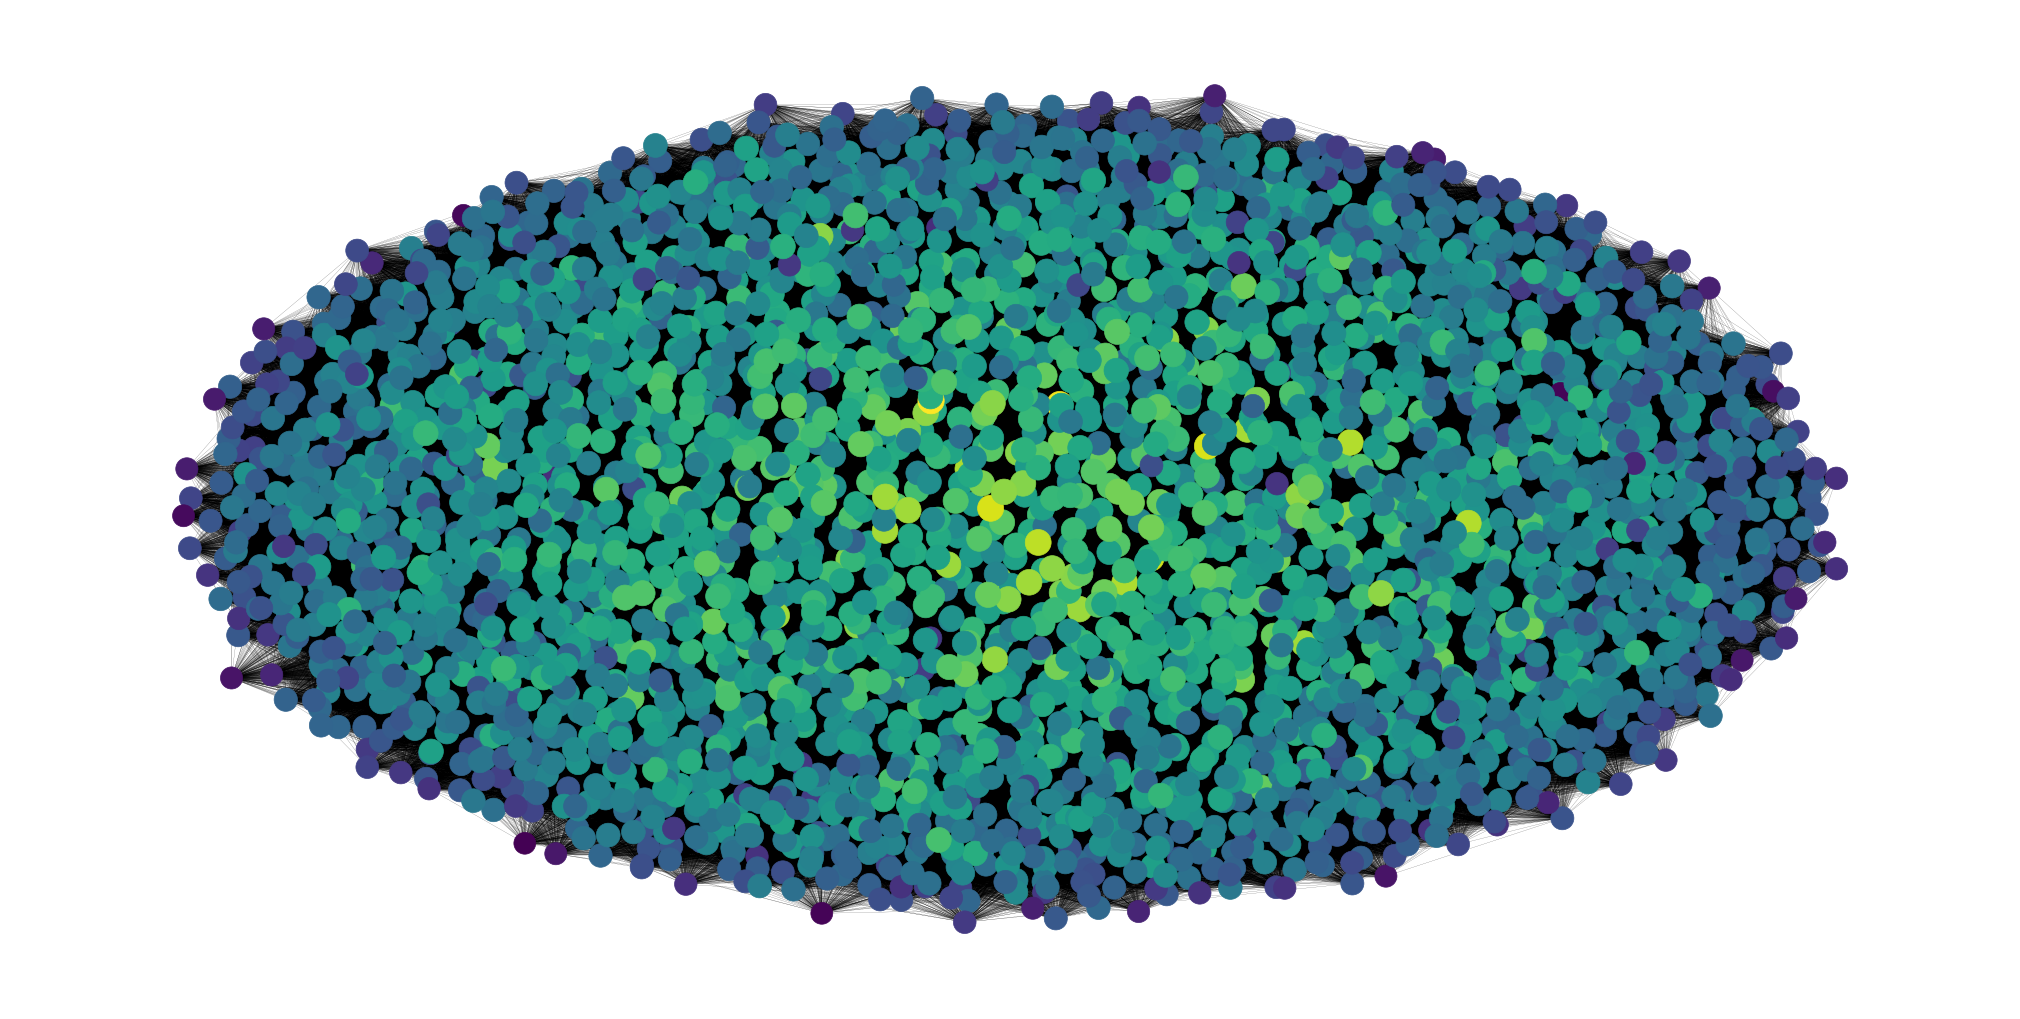
\includegraphics{./assets/3000_draw.png}
  \caption{Random network of 3000 nodes with \(p\) = 0.1}
  \end{subfigure}
  \hfill  
  \begin{subfigure}{0.4\textwidth}
  \centering
  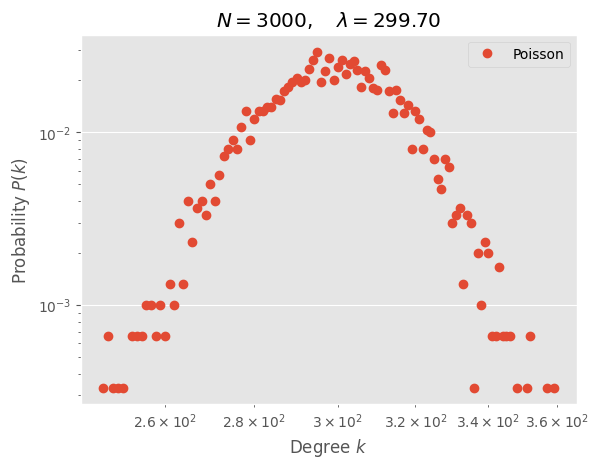
\includegraphics{./assets/3000_poisson.png}
  \caption{Distribution of node degree}
  \end{subfigure}
\end{figure}

The Distribution follows closely the expected Poisson, and shows that
the average degree of the nodes is \(\thicksim 300\), in line with our
expectations. The graph clearly shows a highly connected example, and
further analysis will consider networks with lower \(p\) values.

\begin{figure}
  \centering
  \begin{subfigure}{0.4\textwidth}
    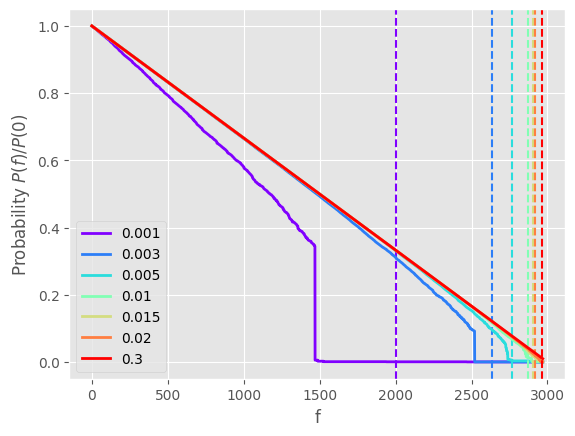
\includegraphics{assets/random_3000.png}
    \caption{Random network failure curves at 3000 nodes}
  \end{subfigure}
  \hfill
  \centering
  \begin{subfigure}{0.4\textwidth}
    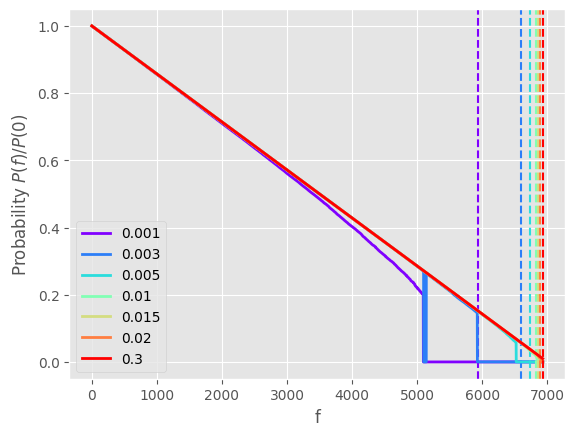
\includegraphics{assets/random_7000.png}
    \caption{Random network failure curves at 7000 nodes}
  \end{subfigure}
\end{figure}

These graphs show how the network responds to randomized failures of its
nodes, up to 99\% of them. We can see that, apart from catastrophic
failures, the trend is one of high resistance of networks, as long as
the probability \(p\) is not too low.

Random graphs show themselves to be quite resistant to node failures,
although under the hypothesis of having enough connections between
nodes. These extra connections act as a backup for the network, allowing
it to keep its structure even under heavy failures.

A clear issue with these models is that random graphs are not likely to
occur in nature or under unconstrained environments, as they often
display a high degree of redundancy, which raises their cost and lowers
their efficiency.

\hypertarget{scale-free-networks}{%
\section{Scale-Free Networks}\label{scale-free-networks}}

As previously stated, random networks are not an effective model for
real world networks. A more recent model that tries to bridge this gap
between theory and practice is the Scale Free model, which uses a Power
Law distribution for the degrees of the nodes. This leads to the
existence of a few major Hubs in the networks, which act as the backbone
of the network.

This difference can already give us an idea of the response of the
network against random failures: most nodes are inconsequential to the
overall network connectedness, and only the removal of the major hubs
impacts the network.

Unlike random networks, the critical exponents of scale free models are
not uniquely defined by the topology itself, instead depending on the
degree exponent \(\gamma\) of the Power Law of the network.

This dependency on \(\gamma\) is also reflected on the expected critical
threshold value:

\[
f_c = \begin{cases}
   1-\frac{1}{\frac{\gamma-2}{3-\gamma}k_{min}^{\gamma-2}k_{max}^{3-\gamma}-1} &\text{if } 2 < \gamma < 3 \\
   1-\frac{1}{\frac{\gamma-2}{\gamma-3}k_{min}-1} &\text{if } \gamma > 3
\end{cases}
\]

\hypertarget{impact-of-random-failures-1}{%
\subsection{Impact of random
failures}\label{impact-of-random-failures-1}}

These graphs show the properties of the generated Scale Free networks.

The parameter \(\gamma\) is computed using a fit function to get the
best estimate, and the graphs shows that it maps quite nicely with the
true distribution of the network.

\begin{figure}
  \begin{subfigure}{0.4\textwidth}
    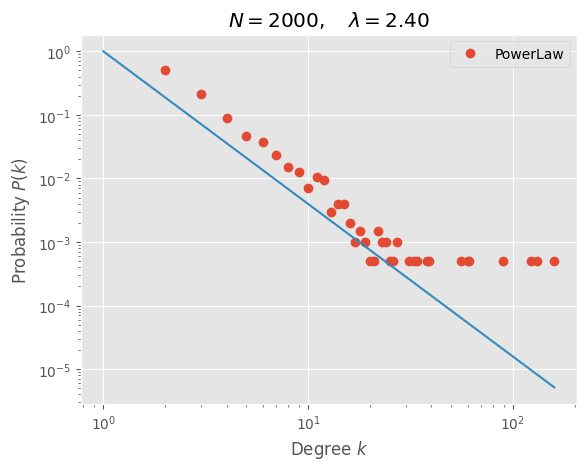
\includegraphics{./assets/2000_lambda_est.png}
  \end{subfigure}
  \hfill
  \begin{subfigure}{0.4\textwidth}
    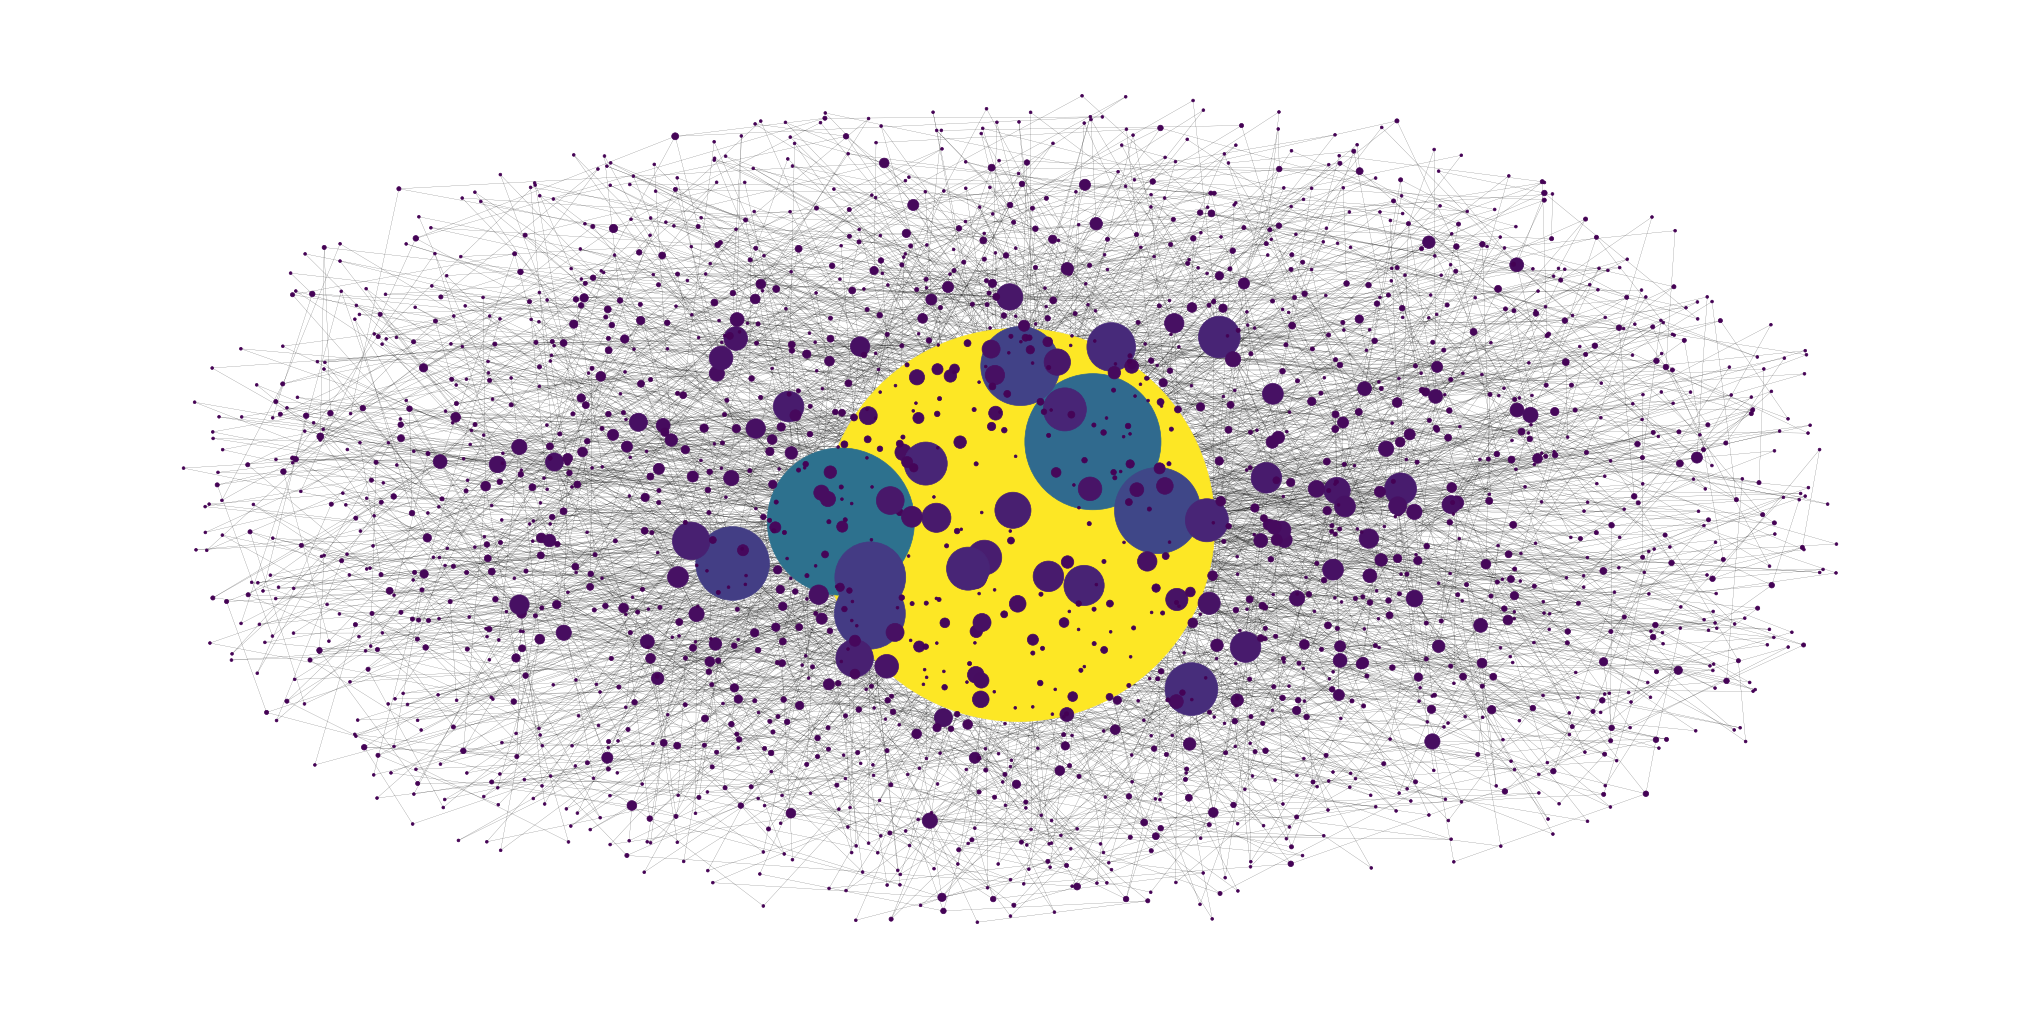
\includegraphics{assets/scalefree_draw.png}
  \end{subfigure}
\end{figure}

The graph visualization also highlights effectively the major roles of
some nodes compared to others. The regular structure we saw in the
random networks is substituted with a strong hierarchy, where a handful
of nodes have a major role in the network.


Here we execute the same node removal algorithm, graphing also the
expected threshold of the networks. We slightly different networks to
get a more general understanding of the problem, alongside different
network sizes to see if any property emerges.

\begin{figure}
  \centering
  \begin{subfigure}{0.3\textwidth}
    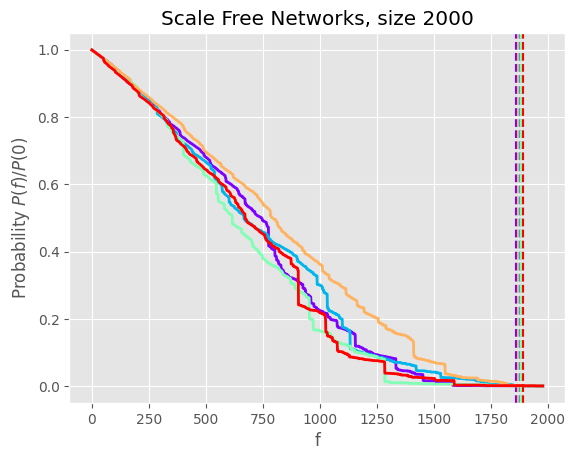
\includegraphics{./assets/scalefree_2000_random.png}
  \end{subfigure}
  \begin{subfigure}{0.3\textwidth}
    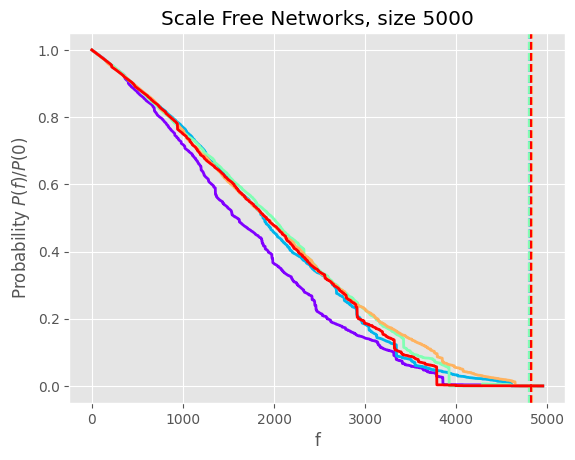
\includegraphics{./assets/scalefree_5000_random.png}
  \end{subfigure}
  \begin{subfigure}{0.3\textwidth}
    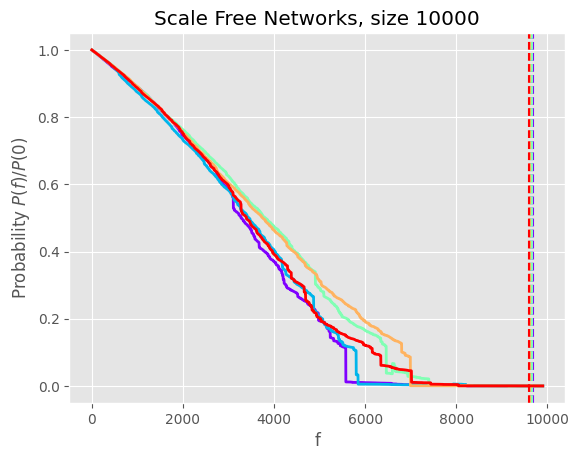
\includegraphics{./assets/scalefree_10000_random.png}
  \end{subfigure}
\end{figure}

We can observe that the networks are less stable compared to the random
ones we saw previously, and we can notice major drops in network
connectivity, likely due to a group of major nodes being removed. The
network is still relatively stable, as a high percentage of nodes has to
fail to cause major damage to the graph, and if the major nodes can be
protected from these failures, we can expect even better performance.

\hypertarget{real-world-networks}{%
\section{Real world networks}\label{real-world-networks}}


\begin{wrapfigure}{R}{0.4\textwidth}
  \centering
  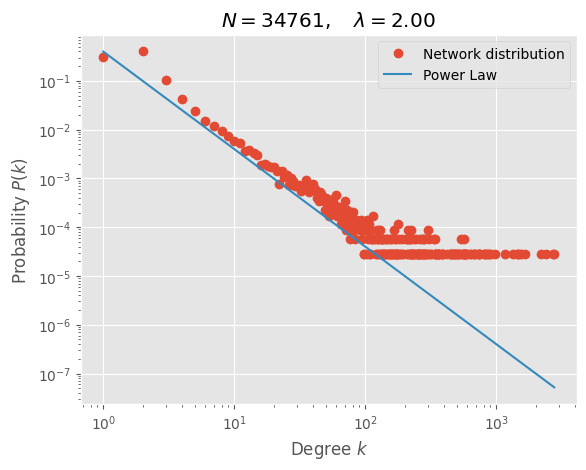
\includegraphics[width=0.4\textwidth]{assets/internet_pl_fit.png}
  \caption{Power Law fit over Topology dataset}
\end{wrapfigure}

As we discussed, the Scale free model resembles much more closely real
world networks, where edges are not simply random, but efficiency is key
and hierarchies are common.

As a model, we decided to use a relatively small internet topology
network, of size \(n = 34761\), obtained from
\href{http://konect.cc/networks/topology/}{konnect}, originally produced
by the \href{http://irl.cs.ucla.edu/}{Internet Research Laboratory, at
UCLA}. The page details many of the network properties, including the
value of the power law exponent at \(\gamma = 2.32\)


\hypertarget{impacts-of-random-failures}{%
\subsection{Impacts of random
failures}\label{impacts-of-random-failures}}


\begin{wrapfigure}{R}{0.4\textwidth}
  \centering
  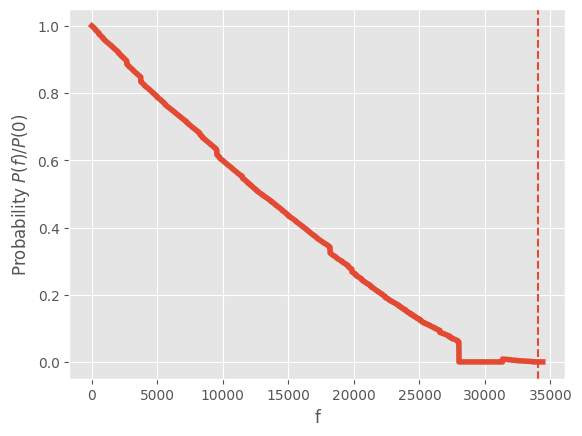
\includegraphics{assets/internet_random_fail_2.png}
  \caption{Internet topology network response to randomized failures}
\end{wrapfigure}

The network shows similar behaviors to its artificial counterparts,
showing good resistance to randomized failures, as most nodes of the
network are inconsequential to the larger connected components. The
computed critical threshold seems also reasonable, reaching into 99\%.

\hypertarget{targeted-failures}{%
\section{Targeted failures}\label{targeted-failures}}

\hypertarget{impacts-on-random-networks}{%
\subsection{Impacts on random
networks}\label{impacts-on-random-networks}}

\hypertarget{impacts-on-scale-free-networks}{%
\subsection{Impacts on scale-free
networks}\label{impacts-on-scale-free-networks}}

\hypertarget{impacts-on-real-world-networks}{%
\subsection{Impacts on real world
networks}\label{impacts-on-real-world-networks}}

\end{document}
